\chapter{Tecnologie Implicate}\label{capitolo2}
In questo capitolo verranno discusse le tecnologie che sono state studiate ed utilizzate durante le attivit\`a di stage.
In particolare il capitolo \`e diviso tra tecnologie hardware e tecnologie software.

\section{Prefazione}
Lo sviluppo del progetto di stage \`e stato svolto nell'ambiente Raspbian\cite{Raspbian}
una distribuzione Debian\cite{Debian} che gira sul dispositivo RasperryPi\cite{Raspberry}.
Inoltre sono state adottate diverse tecnologie nel campo del riconoscimento vocale e di
immagini (OpenCV \cite{OpenCV-website} e Google Speech API \cite{GoogleSTT-website}),
nello sviluppo di applicazioni web (Electron \cite{Electron-website}, Node.JS \cite{Node.JS-website},
Express \cite{Express-website}, Mustache \cite{Mustache}) e della gestione dati (MySQL \cite{MySQL}).
Inoltre sono stati adottati diversi linguaggi di programmazione (JavaScript \cite{JavaScript}, Python \cite{Python}).
Inoltre per la gestione distribuita di progetti software e di versionamento del codice \`e
stata usata la piattaforma GitLab \cite{git-website}.

\section{Hardware}
\subsection{RasperryPi}
RaspberryPi \`e un calcolatore elettronico, montato su una singola scheda elettronica,
caratterizzato dal basso costo, dal consumo energetico ridotto e, per le sue
dimensioni ridotte, dalla facile portabilit\`a.
Rilasciato per la prima volta nel 2012 \`e diventato un prodotto utilizzato per una moltitudine
di progetti sia aziendali che casalinghi.
Il modello usato durante lo stage \`e RaspberryPi 3 model B e monta:
\begin{itemize}
\item CPU con architettura Advanced RISC Machine (ARM)
\item 1 porta HDMI
\item 1 porta LAN
\item 1 uscita Aux
\item 4 porte USB
\item 40 pin General Purpose Input/Output(GPIO)
\item 1 scheda di rete wireless
\item Alimentazione microUSB 5V
\item un bus camera serial interface(CSI), ovvero una porta per telecamera con Flexible flat cable(FFC)
\item ingresso per microSD
\end{itemize}
Il sistema operativo per Raspberry deve essere installato su una microSD opportunamente formattata
e configurata con un Master Boot Record (MBR).

\subsection{Periferiche}
Nella creazione delle applicazioni per il Magic Mirror sono state usate diverse periferiche, tra cui un microfono
USB, per catturare la voce in input e un componente Skydriver Touch Board (94mm x 122mm) di Piromoni collegabile tramite
i 40 pin GPIO del calcolatore principale, per catturare input fisici tramite il movimento delle dita sulla Touch Board.

\section{Software}
\subsection{Raspbian}
Raspbian \`e una distribuzione del sistema operativo Linux derivata da Debian, completamente libera,
ottimizzata per Raspberry.
Fu sviluppata da Mike Thompson e Peter Green come progetto non affiliato alla compagnia RaspberryPi
Fundation, per tenere in considerazione la limitata capacit\`a di calcolo dei processori ARM.
La prima versione venne rilasciata nel 2012.

\subsection{Electron}\label{cap:Electron}
Electron \`e un framework open source rilasciato per la prima volta nel 2013, ma la prima versione
stabile \`e uscita nel giugno 2017. \`E disponibile per i sistemi operativi Windows, MacOS e Linux ed \`e scritto
in C++ e Javascript. Il framework permette la creazione di applicazioni multipiattaforma
utilizzando tecnologie gi\`a esistenti per lo sviluppo
del lato client e del lato server (Javascript, Node.JS, V8 \cite{V8}).
All'avvio di Electron viene inizializzata una pagina con Chromium \cite{Chromium}(un web browser installato insieme all'applicazione)
nel quale viene mostrata una pagina web, e un server in Node.JS.
Un'applicazione sviluppata con Electorn ha bisogno di 3 componenti principali:
\begin{itemize}
\item Il package.json, un file JSON, che deve contenere almeno il nome dell'applicazione,
la versione dell'applicazione creata, la descrizione di quest'ultima e il
 nome del file principale dell'applicazione (necessaria per l'avvio), come mostrato nella
 seguente immagine:
\begin{lstlisting}
{
  "name": "magicmirror",
  "version": "2.1.1",
  "description": "The open source smart platform",
  "main": "js/electron.js"
}
\end{lstlisting}
\emph{Name} \`e il campo che assegna il nome dell'applicazione, \emph{version} \`e il campo che assegna la versione
dell'applicazione, \emph{description} \`e una stringa che descrive il programma, \emph{main} \`e il campo che punta al file
Javascript da eseguire all'avvio.
\item Un file HTML che contiene il template della pagina generata dall'applicazione
\item Un file JavaScript che contiene il codice di esecuzione dell'applicazione come ad esempio la
creazione di una finestra o la visualizzazione di una pagina.
\end{itemize}

\subsection{OpenCV}
OpenCV (Open Source Computer Vision Library) \`e una libreria software sviluppata intorno al 2000
utilizzata nell'ambito della visione artificiale per l'acquisizione e il riconoscimento di immagini
da parte di una macchina per mezzo di input digitali, ottenuti tramite telecamera o fotocamera.\\
La libreria \`e disponibile per i linguaggi C++(linguaggio in cui \`e scritta), C, Python e Java e
per diversi sistemi operativi, compresi quelli specifici per i dispositivi mobili.\\
OpenCV prende in input un'immagine o uno stream (come un video o una serie di immagini) e, utilizzando specifici
algoritmi di Machine Learning, \`e in grado di individuare e riconoscere oggetti specifici.

\subsection{Google Speech API}
Negli ultimi anni Google ha ampliato sempre di pi\`u il suo catalogo per quanto riguarda
i servizi cloud e web API.
Tra questi si pu\`o individuare anche Google Speech API, il quale \`e un
servizio che, ricevendo in input un file o uno stream audio, ottenuto per mezzo di un'acquisizione
da un dispositivo di audio input, traduce il parlato in testo scritto tramite algoritmi avanzati
di riconoscimento della voce.\\
L'API supporta oltre 110 lingue e si possono usare su diverse piattaforme dato che
le librerie sono disponibili nei linguaggi C\#, GO, Java, Node.JS, PhP, Python e Ruby.
Inoltre Google Speech API dispone di alcune varianti:
\begin{itemize}
\item Una con interfaccia REpresentational State Transfer(REST), che comunica per mezzo di URI
\item Una con gRPC, un sistema di chiamata di procedura remota
\end{itemize}

\iffalse
\section{Model-View-Design}
Il Model-View-Design (MVC) \`e un pattern architetturale che suddivide lo sviluppo di un'applicazione web in 3 parti:
\begin{itemize}
\item Model(Modello), sono oggetti che rappresentano lo stato dell'applicazione e operazioni logiche da eseguire sul primo. Di solito
lo stato del modello viene estratto, manipolato per mezzo di operazioni e salvato da un database con cui comunicano,
oppure passato al controller.
\item Controller, \`e un'interfaccia che comunica tra il Model, la View e l'Utente. Il suo compito \`e di gestire le richieste dell'utente,
il quale comunica tramite input ed interazioni, utilizzando il modello che rientra nel dominio
dei dati inerente alla richiesta e selezionando una View per il rendering dell'interfaccia utente.
\item View(Visualizzazione), ha il compito di far visualizzare all'utente i dati estratti tramite un'interfaccia grafica, che viene creata
partendo da un modello HTML.\\[2\baselineskip]
\end{itemize}
\begin{figure}[H]
    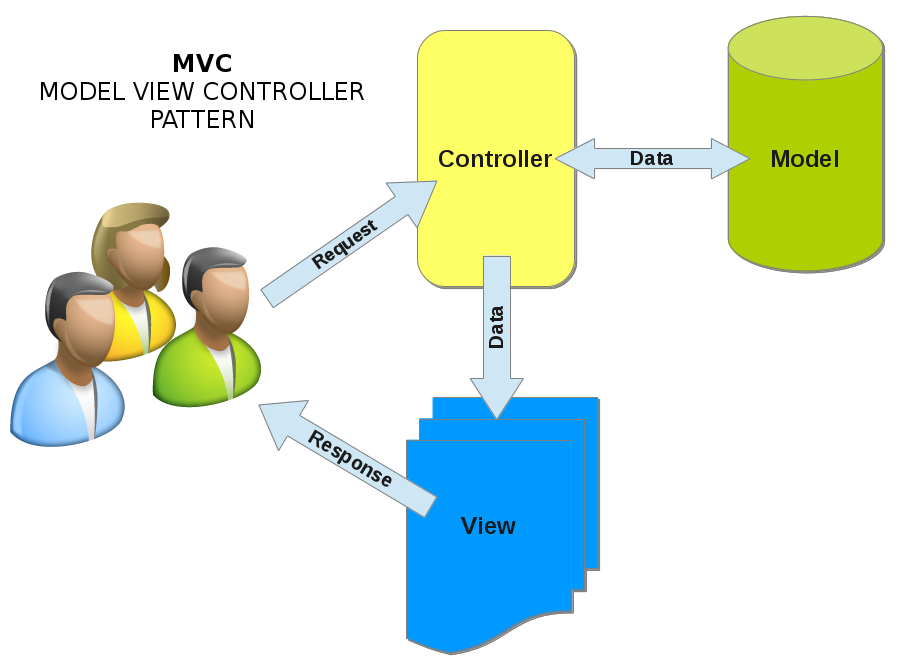
\includegraphics[width=0.9\textwidth]{mvc}
    \caption{MVC Pattern}
\end{figure}
\fi

\subsection{Node.JS}
Node.JS è gi\`a distribuito con Electron, ed \`e stato usato per la creazione del server
per la gestione dell'interfaccia web per il MM.
Node.JS \`e una piattaforma open source che permette l'esecuzione del linguaggio Javascript, sfruttando il motore JavaScript V8 sviluppato da Google,
anche per il lato server, ovvero
la parte del sistema che \`e adibita alla manipolazione e all'elaborazione
dei dati in modo completamente trasparente all'utente.\\
Node.JS esegue delle operazioni al verificarsi di uno specifico evento, che pu\`o essere un accesso ad una porta
del server o la richiesta di una pagina.\\
Per gestire i pacchetti di questo framework viene utilizzato NPM\cite{NPM}, uno strumento che permette
di scaricare ed installare librerie private o pubbliche salvate su un database.
\\[1\baselineskip]

\subsection{Express}\label{cap:express}
Express \`e un framework per Node.JS che permette di creare applicazioni Web in JavaScript, offrendo strumenti e pacchetti
che implementano pi\`u facilmente tutte le funzionalit\`a offerte da Node.JS.
Il software viene usato per creare e gestire il back-end di un server, che \`e composto da 3 entit\`a importanti:
\begin{itemize}
\item il Controller, che definisce le funzioni associate ad un determinato modello.
\item il Routing, utilizzato per determinare come il server debba rispondere ad un determinato metodo di richiesta,
ricevuta sottoforma di URI, inoltrando la stessa alla funzione del controller del rispettivo modello a cui fa rifermento.
\item i Modelli, creati per ogni entit\`a-oggetto che esiste all'interno del server, ad ognuno dei quali viene associato
un controller. Inoltre, tramite i modelli si accede al database per estrarre i dati e spedirli al controller per
la manipolazione, ricevendoli successivamente modificati e salvandoli, se necessario.
\\[2\baselineskip]
\end{itemize}

\subsection{Mustache}\label{cap:mustache}
Mustache \`e un sistema di template, ovvero un sistema che prendendo in input dati e web template
genera automaticamente pagine web, permettendo cos\`i di riutilizzare elementi statici dei template.
Dal momento che Mustache \`e disponibile in diversi linguaggi tra cui Javascript \`e stato usato per l'interfaccia web di configurazione
del MagicMirror.
Mustache \`e un sistema logic-less perch\`e \`e privo di istruzioni per il controllo del flusso
(come ad esempio l'"if" e l'"else"), quindi tutti i controlli di questo tipo sono data-driven.\\

\subsection{MySQL}
MySQL \`e stato usato durante lo stage come database per l'archiviazione di account di utenti
accreditati all'autenticazione per accedere all'interfaccia web di configurazione del MM.\\
MySQL \`e uno tra i pi\`u famosi database open source sviluppato da Oracle, pi\`u precisamente
\`e sistema per la gestione di basi di dati basato sul modello relazionale.
MySQL \`e composto da una semplice riga di comando e un server web, ma sono implementati anche programmi
per l'amministrazione del database come, ad esempio, il famoso phpMyAdmin.
La prima versione fu rilasciata nel maggio del 1995 sviluppata da Oracle e di propriet\`a di MySQL AB,
distribuito sia con licenza commerciale sia con licenza libera.

\subsection{JavaScript}
Javascript \`e un linguaggio di programmazione ad alto livello orientato agli oggetti e ad eventi, che \`e supportato dalla maggior parte dei browser
per lo scripting delle pagine web, e che supporta la programmazione procedurale.
Inizialmente usato per il lato client ha subito un'evoluzione che lo ha portato ad essere utilizzato per lo sviluppo di back-end e web app.
\\[2\baselineskip]
ECMAJavascript(ES) \`e lo standard di Javascript che negli ultimi anni ha sviluppato ed evoluto il linguaggio in diverse versioni.
Uno degli aspetti su cui il processo di standardizzazione si è focalizzato \`e la semplificazione della gestione degli eventi e delle funzioni asincrone
(cio\`e di quelle che riconsegnano il controllo al chiamante prima della loro terminazione).
Le pratiche utilizzate per sincronizzare di queste funzioni in ECMAJavascript 5 (ES5), la versione usata durante lo
stage, sono l'utilizzo delle callback.\\[1\baselineskip]
In ECMAJavascript 6 (ES6) \`e stato introdotto il concetto di Promises, che ha sostituito le funzioni di Callback.
Una Promise rappresenta un proxy per un valore non necessariamente noto quando la Promise è stata creata. Consente di associare degli handlers
con il successo o il fallimento di un'azione asincrona (e il "valore" in caso di successo, o la motivazione in caso di fallimento).
Sono tutt'ora in via di sviluppo nuove versioni di Javascript.

\subsection{Python}\label{cap:python}
Python \`e un linguaggio di programmazione open source, ad alto livello con semantica dinamica, orientato ad oggetti, usato
per sviluppo di applicazioni e scripting.\\[1\baselineskip]
Questo linguaggio \`e stato particolarmente utile per l'interfacciamento con la telecamera e la Touch Board, essendo a disposizione librerie
apposite per gestirle.\\
Come molti altri linguaggi supporta l'implementazione di pacchetti esterni che possono essere salvati in una repository pubblica
o su piattaforme esterne.
Nel primo caso Python utilizza un suo gestore di pacchetti: Pip Installs Packages o Pip Installs Python (pip, acronimo ricorsivo).
Nel secondo caso i pacchetti possono essere inseriti senza dover utilizzare il gestore di pacchetti appena introdotto.
\\[2\baselineskip]

\subsection{GitLab}
GitLab \`e una piattaforma web che implementa le funzionalit\`a offerte dal software Git e altri
servizi tra i quali la possibilit\`a di creare wiki e un servizio di issue tracking, utile per tenere traccia
di eventuali richieste o problemi.
La comodit\`a di questa piattaforma sta nel poter creare dei Commit, ovvero ad ogni modifica del codice si pu\`o
salvarne lo stato assegnandoli un'etichetta in locale, per poi spedirlo al respository in remoto del progetto.
In ogni momento si pu\`o tornare ad una versione vecchia tramite gli strumenti di versionamento offerti dalla piattaforma web.
